%!TEX root = theorie_solfege_Bxl.tex
\chapter{La mesure}\index{mesure}

\section{La pulsation et le temps}\index{pulsation}
\subsubsection{La pulsation}
La pulsation est un battement régulier, un peu comme les battements de c\oe{}ur. Elle marque le début de chaque temps. La succession des pulsations indique la durée des temps ainsi que le tempo.
\subsubsection{Le temps}\index{temps}
Le temps est la durée entre une pulsation et la suivante.
\subsubsection{La tempo}\index{tempo}
Le tempo correspond à la vitesse à laquelle les pulsations se suivent.

\section{La battue de mesure}\index{battue}
Le mouvement est très important: il nous permet de savoir et de sentir sur quel temps de la mesure nous nous trouvons. Dans un orchestre, il permet aux musiciens de savoir quand il vont devoir commencer à jouer. Le premier temps est \emph{toujours} vers le bas.

\subsubsection{Mesure à 2 temps}
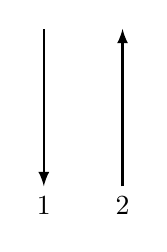
\begin{tikzpicture}
\draw [thick, latex-] (0,0) -- (0,2) node [below=2cm]{1}; 
\draw [thick, -latex] (1,0) -- (1,2) node [below=2cm]{2}; 
\end{tikzpicture}

\subsubsection{Mesure à 3 temps}
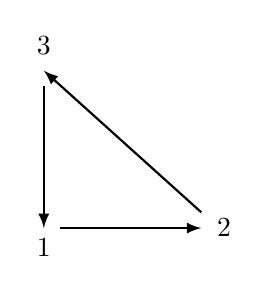
\begin{tikzpicture}
\draw [thick, latex-] (0,0) -- (0,1.8) node [below=1.8cm]{1}; 
\draw [thick, -latex] (0.2,0) -- (2,0) node [right=2pt]{2}; 
\draw [thick, -latex] (2,0.2) -- (0,2) node [above=2pt]{3}; 
\end{tikzpicture}

\subsubsection{Mesure à 4 temps}
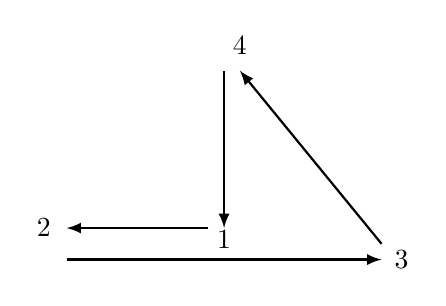
\begin{tikzpicture}
\draw [thick, latex-] (2,0) -- (2,2) node [below=1.9cm]{1}; 
\draw [thick, -latex] (1.8,0) -- (0,0) node [left=2pt]{2}; 
\draw [thick, -latex] (0,-0.4) -- (4,-0.4) node [right=1pt]{3}; 
\draw [thick, -latex] (4,-0.2) -- (2.2,2) node [above=2pt]{4}; 
\end{tikzpicture}

Il existe d'autres mouvements de mesures (6 temps lents, 5 temps), mais on les utilise rarement.

\section{Mesures binaires et ternaires}
\subsection{Mesures binaires}\index{binaire}
Les mesures binaires sont les mesures dont les temps sont divisibles par 2: \lilyTimeSignature{2}{4}, \lilyTimeSignature{3}{4}, \lilyTimeSignature{4}{4}, etc. On les appelle aussi \emph{mesures simples}.\index{mesure simple}

\subsection{Mesures ternaires}\index{ternaire}
Les mesures ternaires sont les mesures dont les temps sont divisibles par 3: \lilyTimeSignature{6}{8}, \lilyTimeSignature{9}{8}, \lilyTimeSignature{12}{8}, etc. Même si \lilyTimeSignature{6}{8} indique une mesure de 6 croches, il ne s'agit généralement pas d'une mesure à 6 temps (sauf en tempo lent), mais d'une mesure à 2 temps, chaque temps valant 3 croches (ou une noire pointée). On les appelle aussi \emph{mesures composées}.\index{mesure composée}


%\subsubsection{Mesure à 6 temps}
%\begin{tikzpicture}
%\draw [thick, latex-] (2,0) -- (2,2) node [below=1.9cm, left=2pt]{1}; 
%\draw[thick, ->] (2.1,0) arc (180:0:8pt) node [below=-0.7cm]{2};
%\draw[thick, ->] (2.9,0) arc (180:0:8pt) node [below=-0.7cm]{3};
%\draw [thick, -latex] (3.6,-0.2) -- (0,-0.2) node [left=2pt]{4}; 
%\draw [thick, -latex] (0,-0.5) -- (4.5,-0.5) node [right=1pt]{5}; 
%\draw [thick, -latex] (4.5,-0.3) -- (2.2,2) node [above=2pt]{6}; 
%\end{tikzpicture}

%\subsubsection{Mesure à 5 temps}
%\begin{tikzpicture}
%\draw [thick, latex-] (2,0) -- (2,2) node [below=1.9cm, right=2pt]{1}; 
%\draw[thick, ->] (1.9,0) arc (0:180:8pt) node [below=-0.7cm]{2};
%\draw[thick, ->] (1.2,0) arc (0:180:8pt) node [below=-0.7cm]{3};
%\draw [thick, -latex] (0.5,-0.2) -- (4.5,-0.2) node [right=1pt]{4}; 
%\draw [thick, -latex] (4.5,0) -- (2.2,2) node [above=2pt]{5}; 
%\end{tikzpicture}

\section{La barre de reprise}
Pour indiquer qu'il faut répéter une ou plusieurs mesures, on utilise parfois des barres de reprises. Toutes les mesures comprise entre 2 barres de reprises (ou entre le début et une barre de reprise) doivent être rejouées. Cela permet de ne pas devoir ré-écrire un passage complet et d'économiser de la place.

\includegraphics{exemples/reprise}

\section{Les chiffres de mesure}\index{chiffres de mesure}
Les chiffres de mesure comptent toujours 2 nombres:
\begin{itemize}
\item le premier (au-dessus) indique le nombre de pulsations par mesure
\item le deuxième (en-dessous) indique la valeur de chaque pulsation
\end{itemize}


Pour savoir à quelle valeur correspond le deuxième nombre, on divise une ronde comme dans le tableau des valeurs de notes (page \pageref{tableaunotes}):
\begin{itemize}
\item 1 = une ronde
\item 2 = une blanche (la moitié d'une ronde)
\item 4 = une noire (le quart d'une ronde)
\item 8 = une croche (le huitième d'une ronde)
\end{itemize}
Une mesure \lilyTimeSignature{2}{4} indique donc 2 temps par mesure, chaque temps valant une noire. Une mesure \lilyTimeSignature{2}{2} indiquera aussi 2 temps par mesure, mais chaque temps vaudra alors une blanche.

